\documentclass[10 pt]{article}
\usepackage{graphicx}
\pagestyle{plain}
\usepackage[OT4]{polski}
\usepackage[utf8]{inputenc}
\title{Sprawozdzanie 8 \\ \emph{\textbf{Grafy v1.5}}}
\author{Paweł Żurek 200404}
\date{14.0.2014}
\begin{document}
\tableofcontents
\maketitle
\section{Wstęp}
Prosty program, w którym użyte są podstawowe funkcje grafów.
\section{Krótki opis programu}
\textbf{Program po uruchomieniu pyta się z ilu wierzchołków ma stworzyć graf a następnie udostępnia proste menu : }
\begin{itemize}
\item Ustawienie połączeń między wierzchołkami
\item Dodanie wierzchołka
\item Usunięcie wierzchołka
\item Dodanie krawędzi
\item Usunięcie krawędzi
\item Wyświetlenie sąsiadów wierzchołka
\item Wyświetlenie grafu ( za pomocą macierzy połączeń )
\item Podanie ilości wierzchołków
\item Wyświetlenie aktualnych wierzchołków
\item Algorytm Depth First Search
\item Algorytm Breadth First Search
\item Losowanie połączeń wraz z ich wagami
\item Algorytm A* ( A star )
\end{itemize}
Jako, że zaimplementowałem strukturę grafu za pomocą macierzy połączeń, najważniejszym elementem mojego programu jest : 
\begin{itemize}
\item Macierz typu int ( tablica dynamiczna dwu wymiarowa ) przechowująca aktualne połączenia między wierzchołkami
\end{itemize}
W tej wersji programu uwagę skupiłem na algorytmach \textbf{dfs}, \textbf{bfs} i \textbf{A*}. Dlatego też tym algorytmom będzie poświęcona dalsza część sprawozdania.

\section{\textbf{DFS} vs \textbf{BFS}}
Algorytm Depth First Search działa poprawnie. Jako argument, funkcja przyjmuje dowolny wierzchołek, od którego zacznie przeszukiwanie. Wynikiem funkcji jest ciąg wierzchołków połączonych w pośredni lub bezpośredni sposób z wierzchołkiem przyjętym jako argument funkcji.
\\
Algorytm Breadth First Search również działa poprawnie. Mimo tego, że oba algorytmy posiadają inną metodę działania, działanie funkcji wywołującej oba algorytmy jest dokładnie taki sam.
\subsection{Wyniki : }
\begin{center}
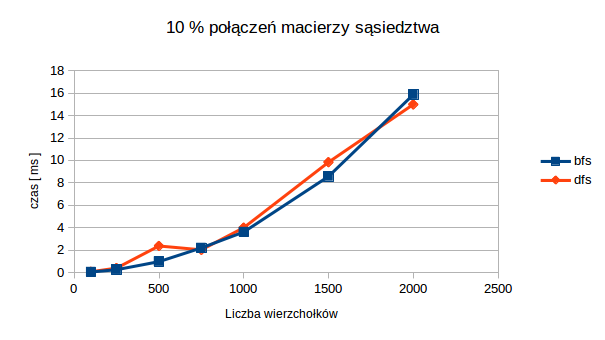
\includegraphics[scale=0.7]{10.png}
\end{center}
\begin{center}
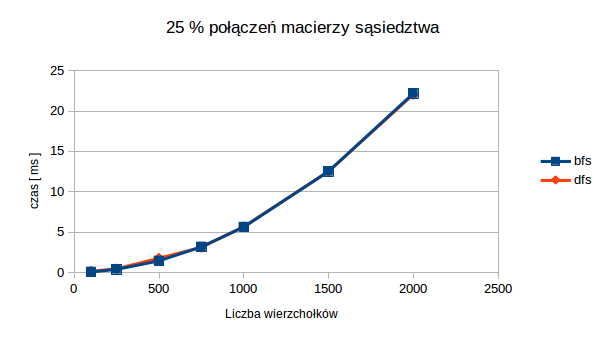
\includegraphics[scale=0.7]{20.png}
\end{center}
\begin{center}
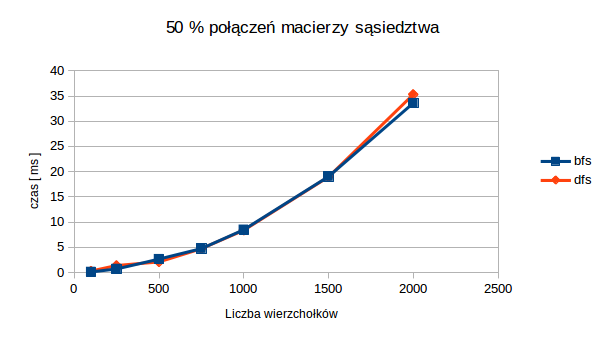
\includegraphics[scale=0.7]{50.png}
\end{center}
\begin{center}
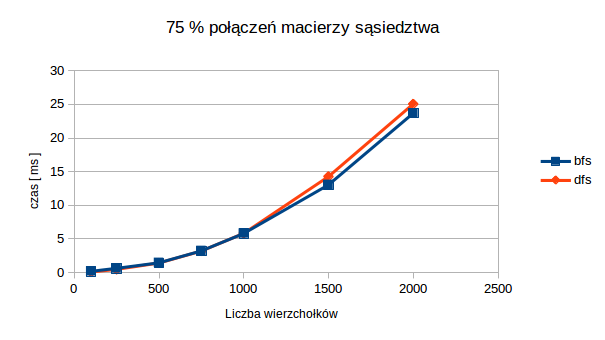
\includegraphics[scale=0.7]{75.png}
\end{center}
\begin{center}
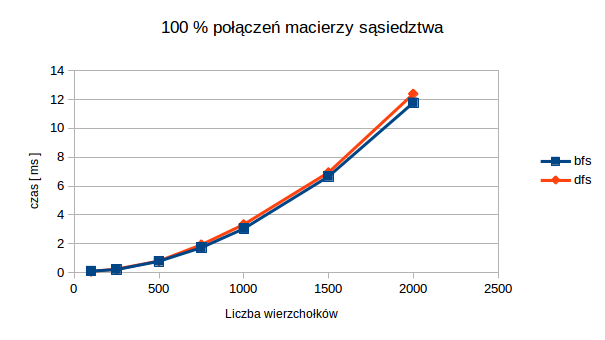
\includegraphics[scale=0.7]{100.png}
\end{center}
\subsection{Uwagi :}
\begin{itemize}
\item Zarówno algorytm \textbf{bfs} jak i algorymt \textbf{dfs} uruchamiałem z tym samym argumentem : wierzchołkiem o numerze 1.
\end{itemize}
\section{Algorytm \textbf{A*}}
Na dzień dzisiejszy ( 14.05.2014 ) algorytm ten nie działa poprawnie. Jest to głównie spowodowane trudnościami w przejściu z struktur opisanych w materiałach znalezionych w sieci lub literaturze na strukturę, którą operuję. We wszystkich spotkanych mi materiałach, algorytm ten jest stosowany, dla struktur dwu wymiarowych i szukania na nich połączenia. W moim programie, ciężko przedstawić w taki sposób zbiór wierzchołków. 
\\
Algorytm jest zupełny i optymalny, w tym sensie, że znajduje ścieżkę, jeśli tylko taka istnieje, i przy tym jest to ścieżka najkrótsza. Stosowany głównie w dziedzinie sztucznej inteligencji do rozwiązywania problemów i w grach komputerowych do imitowania inteligentnego zachowania.
\section{Wnioski:}
\begin{itemize}
\item Algorytm \textbf{dfs} jest znacznie prostszy w implementacji niż \textbf{bfs}. Przynajmniej w mojej wersji grafu
\item Czasy wykonywania algorytmów \textbf{bfs} i \textbf{dfs} są bardzo zbliżone ( na tyle, że nie jestem pewien czy program dobrze działa ). Częsciej mniejsze czasy są dla \textbf{dfs}, lecz tak małe różnice ( na poziomie milisekund ) mogą być spowodowane obsługą innych procesów w tle procesora.
\item algorytm \textbf{A*} jest prawdopodobnie najefektywniejszym algorytmem tego typu. Dzieje się tak głównie poprzez fakt, iż algorytm na bieżąco ''przewiduje'', która ścieżka jest optymalna.  
\end{itemize}

Dokładne wyniki programu są zamieszczone w pliku ( obecny folder ) wykresy.xls. Podobnie wszystkie wykresy są dostępne w osobnych plikach ( format png ).

\end{document}